\documentclass[11pt]{article}

\usepackage[margin=1in]{geometry}
\usepackage{booktabs}
\usepackage{graphicx}
\usepackage{amsmath}
\usepackage{caption}
\usepackage[hidelinks]{hyperref}

\newcommand{\su}{\textit{SU}}

\title{Generic Drug Prices and the Number of Firms:\\
Preliminary Descriptive Analysis}
\author{PricingEntry project}
\date{July 15, 2026}

% Numbers in this report are from the July 15, 2026 runs of
% clean_prices.do, build_molecule_panel.do, link_diagnostics.do,
% desc_ngen_trajectories.do, and price_hysteresis.do.

\begin{document}
\maketitle

\begin{abstract}
\noindent We document how generic drug prices in the United States co-move
with the number of generic suppliers, using IQVIA quarterly data for
2004--2019. There are three preliminary findings. First, the trajectory of the generic firm count
within a molecule commonly follows a rise--peak--decline pattern: among
molecules whose count peaks at three or more firms, roughly one third lose at
least half of their suppliers by the end of the sample, and only one in ten
remains at its peak. Second, generic prices move asymmetrically over this
cycle: molecules with substantial firm-count declines see average generic
prices \emph{rise} by about 0.9--1.2 log points from the peak year onward,
whereas prices are flat where counts hold. Third, the price reversal after
exit is incomplete: comparing periods with the same number of firms before
and after the peak, and controlling for aggregate trends, roughly half of
the competitive price reduction achieved at the peak persists after the firm
count falls back (``price hysteresis''), with a conservative lower bound of
about one quarter.
\end{abstract}

\section{Data and panel construction}

\paragraph{Source data.} Four IQVIA extracts of US sales at the
country--sector--corporation--product--pack--quarter level: 2004--2008,
2009--2010, 2011--2016 (Excel), and 2017--2019 (csv). Each records
manufacturer revenue (LCD~MNF, equal to USD for the US) and standard units.
Standard units (\su) are pack-size adjusted 
valid.

\paragraph{Cleaning.} We keep single-ingredient products (fixed-dose
combinations are dropped). Each extract is collapsed to cells defined
by corporation $\times$ molecule $\times$ strength $\times$ quarter,
separately for branded and generic products. A product is classified generic
if (a) its name contains the molecule name, (b) its first word is a
truncation of the molecule name, (c) it carries IQVIA's
unbranded-commodity suffix (STCE), or (d) its first word is shared by three
or more corporations within the molecule, which catches drug abbreviations
(HCTZ) and store-brand OTC names, or (e) its name contains the
corporation's name or 4-character code (MKES = McKesson) and its first word
is shared by two or more corporations.
The four cleaned segments are appended into a panel of 1{,}110{,}905 cells.
Branded products account for 31\% of cells but 87\% of revenue (\$4.23T of
\$4.85T).

\paragraph{Molecule panel.} The analysis panel collapses to
molecule~$\times$~quarter, excluding IQVIA's catch-all pseudo-molecules
(diagnostic kits, medical devices, cream bases, ``composition unknown''):
97{,}608 observations on 2{,}210 molecules, 2004Q1--2019Q4
($\approx$1{,}450--1{,}650 molecules active per quarter).
Table~\ref{tab:sumstats} reports summary statistics. Firm counts are counts
of distinct corporations with positive sales; prices are revenue per
standard unit. The counts suggest that we might still have misclassified some generic products as branded (more data work needed). 

\begin{table}[htbp]
\centering
\caption{Molecule--quarter panel: summary statistics}
\label{tab:sumstats}
\begin{tabular}{lrrrrr}
\toprule
 & Obs. & Mean & Std.\ dev. & Min & Max \\
\midrule
No.\ generic firms        & 97{,}608 & 3.33 & 5.39 & 0 & 43 \\
No.\ branded firms        & 97{,}608 & 1.56 & 2.13 & 0 & 34 \\
Generic price (\$/\su)    & 51{,}946 & 23.4 & 165.2 & 0.001 & 7{,}579 \\
Branded price (\$/\su)    & 83{,}395 & 394.9 & 9{,}820 & 0.001 & 2{,}054{,}926 \\
\bottomrule
\end{tabular}
\par\smallskip
\parbox{0.92\textwidth}{\footnotesize Notes: One observation is a
molecule--quarter. Prices are total revenue divided by total standard
units, defined when the corresponding volume is positive. Molecules with
many branded firms are over-the-counter products with genuinely many brand
names (e.g.\ diphenhydramine: Benadryl, Unisom, Nytol); prescription
molecules almost always have at most one or two.}
\end{table}

\section{Linking the four extracts}

Firm names are stamped with the corporate structure as of each extract's
pull date, and pull dates are not chronological across extracts. Firm-level linking across extracts is
therefore unreliable, while molecule-level aggregates are clean.
Table~\ref{tab:linking} quantifies this: apparent exit rates of
firm--molecule--strength cells jump an order of magnitude at the three
extract boundaries relative to identical seasonal transitions within
extracts, with mirror-image entry spikes. At the molecule level, by
contrast, coverage moves smoothly, within-molecule changes in generic firm
counts show only small boundary effects (mean $\Delta n$ of $-0.26$ to
$+0.20$ at boundaries vs.\ about $+0.05$ at normal Q4$\to$Q1 transitions), and
generic price changes at boundaries are indistinguishable from normal
quarters. The analysis is accordingly conducted at the molecule level, and
event-style analyses treat the three boundary transitions as
non-informative.

\begin{table}[htbp]
\centering
\caption{Apparent exit and entry rates at extract boundaries}
\label{tab:linking}
\begin{tabular}{lcc}
\toprule
Transition (Q4$\to$Q1) & Exit rate & Entry rate \\
\midrule
2008Q4 $\to$ 2009Q1 (boundary) & 0.444 & 0.407 \\
2010Q4 $\to$ 2011Q1 (boundary) & 0.237 & 0.264 \\
2016Q4 $\to$ 2017Q1 (boundary) & 0.365 & 0.337 \\
\addlinespace
Mean, 12 within-extract Q4$\to$Q1 & 0.028 & 0.039 \\
Mean, all non-boundary quarters   & 0.030 & --    \\
\bottomrule
\end{tabular}
\par\smallskip
\parbox{0.92\textwidth}{\footnotesize Notes: Cells are
corporation--molecule--strength combinations with positive standard units.
Exit: active in $t$, not active in $t+1$. Entry: active in $t$, not in
$t-1$ (dated by the quarter entered). Boundary spikes reflect IQVIA's
retroactive renaming of corporations, not real firm turnover.}
\end{table}


\section{Trajectories of the generic firm count}

Is rise--peak--substantial-decline a common firm-count trajectory? For each
molecule we compute annual firm counts (the maximum across the year's
quarters, which absorbs boundary noise), the peak count, and the
end-of-sample count. Table~\ref{tab:classes} classifies molecules. Among the
497 ``judgeable'' molecules---peak of at least 3 generic firms, reached at
least three years before the end of the sample, observed through 2019---the
median molecule ends at 67\% of its peak count; one third lose at least
half their suppliers; only 10\% remain at peak. The peak follows a genuine
rise (median $+2$ firms relative to the first observed year, mean $+4.3$;
73\% of peaks are interior). Declines are strongly concentrated in smaller
markets: 54\% of molecules peaking at 3--5 firms fall substantially, versus
16\% of those peaking at 11+. Excluding vitamins/minerals (ATC A11/A12)
changes nothing.

\begin{table}[htbp]
\centering
\caption{Trajectory classification of generic firm counts, by molecule}
\label{tab:classes}
\begin{tabular}{lrr}
\toprule
 & Molecules & Share \\
\midrule
No generics ever                    &   975 & 44.1\% \\
Low activity (peak 1--2 firms)      &   381 & 17.2\% \\
Leaves sample before 2019           &    60 &  2.7\% \\
Peak $<$3 years before end (censored) & 297 & 13.4\% \\
\addlinespace
\emph{Judgeable (peak $\geq 3$, $\geq$3y post-peak):} & 497 & \\
\quad Substantial fall (end $\leq$50\% of peak) & 170 & 34.2\% \\
\quad Moderate fall (50--75\%)                  & 139 & 28.0\% \\
\quad Small fall (75--99\%)                     & 137 & 27.6\% \\
\quad No fall (ends at peak)                    &  51 & 10.3\% \\
\bottomrule
\end{tabular}
\par\smallskip
\parbox{0.92\textwidth}{\footnotesize Notes: Annual firm count = maximum
over the year's quarters. Shares in the top panel are of all 2{,}210
molecules; shares in the bottom panel are of the 497 judgeable molecules.
Molecules that leave the sample entirely (the ultimate fall) are kept as a
separate category, so the fall rates below are conservative.}
\end{table}

Two checks confirm the declines are real rather than artifacts of the
extract seams. First, within the single-vintage 2011--2016 extract
(molecules peaking 2011--13, observed through 2016), the median molecule
ends at 80\% of peak over just a three-year window, with 12\% at
$\leq$50\%. Second, the event-time profile around interior peaks
(Figure~\ref{fig:peak}) shows a symmetric climb from 43\% of peak six years
before to the peak, followed by a decline to 69\% six years after.

\begin{figure}[htbp]
\centering
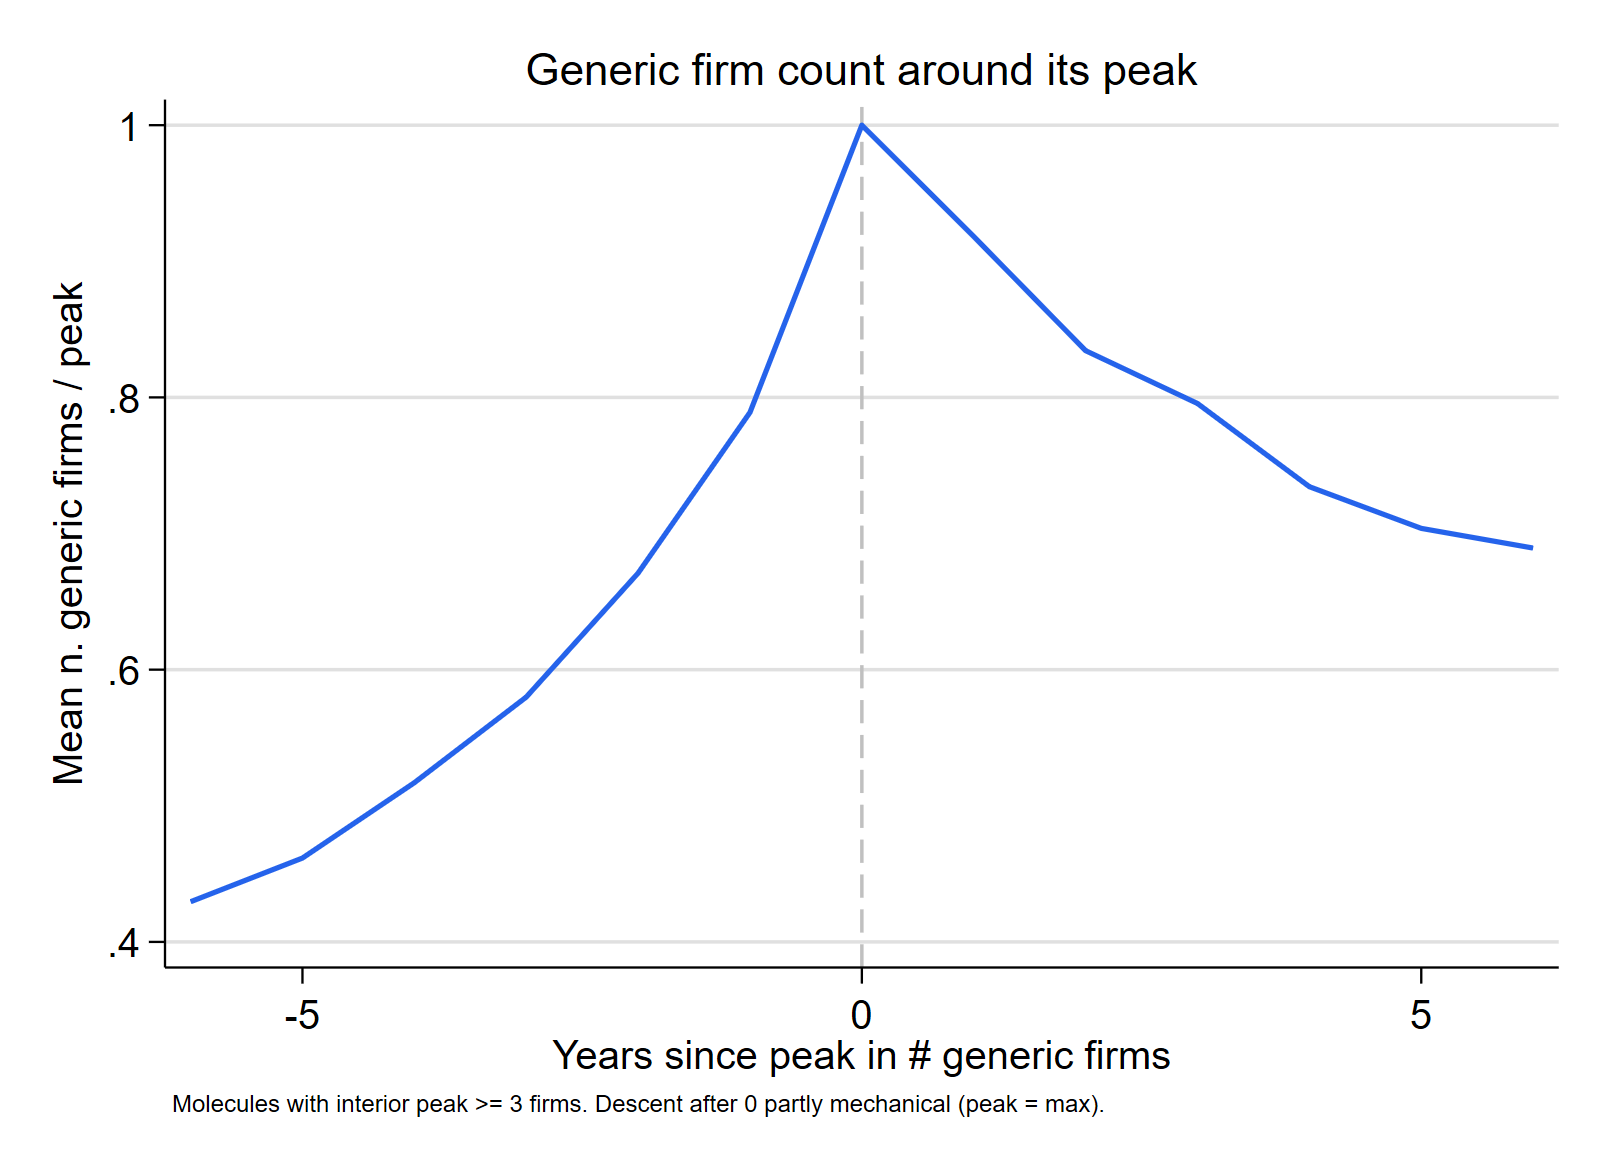
\includegraphics[width=0.72\textwidth]{../output/fig_peak_eventtime.png}
\caption{Generic firm count around its peak (interior peaks $\geq 3$ firms;
count normalized by the molecule's peak).}
\label{fig:peak}
\end{figure}

A cleaner cohort view aligns molecules at their \emph{first} generic entry
(260 episodes in 2006--2015 with a branded incumbent and at least one
generic-free year of prior history; no mechanical peak alignment). The mean
firm count rises from 2.3 at entry to 6.1 after four years and is still
rising at that horizon, while the median generic price falls to 48\% of its
at-entry level (Figure~\ref{fig:cohort}). Declines thus typically arrive
later in the market's life cycle, though 15\% of these young cohorts have
already lost half of their peak count within four years.

\begin{figure}[htbp]
\centering
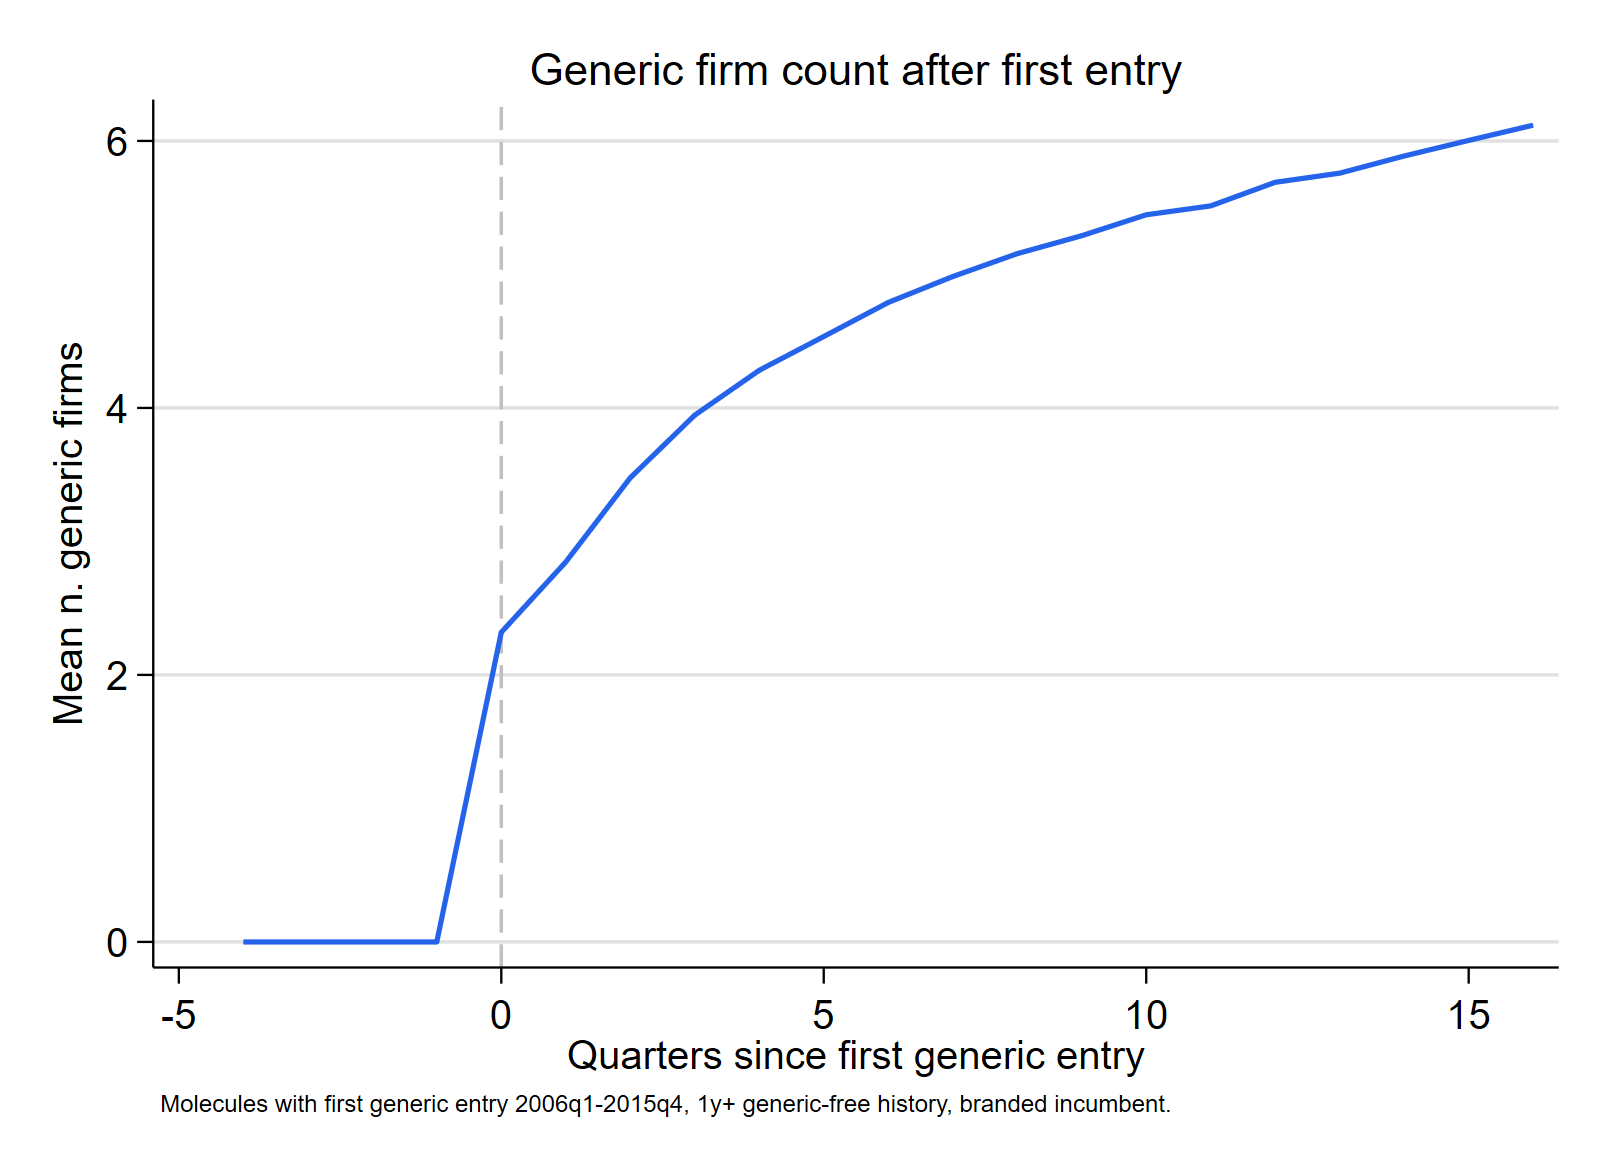
\includegraphics[width=0.72\textwidth]{../output/fig_entry_cohort.png}
\caption{Generic firm count after the first generic entry (mean across 260
molecules; entries 2006Q1--2015Q4).}
\label{fig:cohort}
\end{figure}

\section{Price patterns around firm-count declines}

\subsection{Prices rise where counts collapse}

Table~\ref{tab:pricefall} relates the change in the average generic price
from the peak year to the end of the sample to the trajectory class.
Molecules with substantial firm-count declines see generic prices rise by a
median 0.87 log points (mean 1.24); where counts hold, prices are flat to
declining. The gradient is monotone.

\begin{table}[htbp]
\centering
\caption{Change in log generic price, peak year $\to$ last year, by class}
\label{tab:pricefall}
\begin{tabular}{lrrrr}
\toprule
Trajectory class & $N$ & Mean & Median & p75 \\
\midrule
Substantial fall & 149 & $1.24$  & $0.87$  & $1.87$ \\
Moderate fall    & 139 & $0.27$  & $-0.06$ & $0.75$ \\
Small fall       & 137 & $0.10$  & $-0.16$ & $0.25$ \\
No fall          &  51 & $0.13$  & $-0.08$ & $0.23$ \\
\bottomrule
\end{tabular}
\par\smallskip
\parbox{0.92\textwidth}{\footnotesize Notes: Judgeable molecules with
defined prices in both the peak and final year. Prices are average revenue
per standard unit across the molecule's generic products.}
\end{table}

Several of the largest substantial-fall molecules by revenue are known
regulatory episodes---colchicine (13$\to$6 firms, price $+4.5$ log points),
vasopressin (5$\to$0), pancrelipase (4$\to$0), all affected by the FDA
Unapproved Drugs Initiative---while others (atenolol 20$\to$10, bicalutamide
12$\to$6, nicardipine 9$\to$4) resemble ordinary competitive shakeouts.
Regulatory removals are thus a quantitatively important and plausibly
exogenous source of exit.

\subsection{The reversal is incomplete: price hysteresis}

If a molecule's firm count rises from 5 to 10 and later falls back to 5,
does the price return to its original 5-firm level? We estimate
\begin{equation*}
\ln p_{mt} \;=\; \alpha_m + \delta_t + \beta \ln n_{mt}
 + \gamma \ln n^{\max}_{mt} + \varepsilon_{mt},
\end{equation*}
where $n_{mt}$ is the current generic firm count and $n^{\max}_{mt}$ its
within-molecule running maximum. Complete reversal implies $\gamma = 0$;
the share of the up-leg price reduction retained after the count returns is
$\gamma/(\beta+\gamma)$. Table~\ref{tab:hysteresis} shows both current and
historical-peak counts matter. The baseline retained share is 0.54 (s.e.\
0.10); allowing molecule-specific linear trends---a conservative
specification, since trends absorb genuine long-run hysteresis---gives an
imprecise 0.27 (s.e.\ 0.16); the peak-$\geq$5 sample gives 0.65. In levels,
the current count is largely priced out ($-0.021$, marginal) while the
historical peak carries $-0.117$ per firm: the competitive effect of the
\emph{current} count is concentrated at low $n$, and history dominates
elsewhere.

\begin{table}[htbp]
\centering
\caption{Price hysteresis: current vs.\ historical-peak firm count}
\label{tab:hysteresis}
\begin{tabular}{lcccc}
\toprule
 & (1) Baseline & (2) Mol.\ trends & (3) Peak $\geq 5$ & (4) Levels \\
\midrule
$\ln n$            & $-0.341$ & $-0.303$ & $-0.304$ &          \\
                   & $(0.066)$ & $(0.052)$ & $(0.092)$ &        \\
$\ln n^{\max}$     & $-0.401$ & $-0.114$ & $-0.575$ &          \\
                   & $(0.088)$ & $(0.076)$ & $(0.119)$ &        \\
$n$                &          &          &          & $-0.021$ \\
                   &          &          &          & $(0.013)$ \\
$n^{\max}$         &          &          &          & $-0.117$ \\
                   &          &          &          & $(0.015)$ \\
\addlinespace
Retained share $\gamma/(\beta{+}\gamma)$
                   & $0.54$   & $0.27$   & $0.65$   & $0.85$   \\
                   & $(0.10)$ & $(0.16)$ & $(0.11)$ & $(0.09)$ \\
\addlinespace
Molecule FE, quarter FE & yes & yes & yes & yes \\
Molecule trends    & no  & yes & no  & no  \\
Observations       & 51{,}926 & 51{,}926 & 34{,}406 & 51{,}926 \\
Molecules          & 1{,}215  & 1{,}215  & 666      & 1{,}215  \\
\bottomrule
\end{tabular}
\par\smallskip
\parbox{0.92\textwidth}{\footnotesize Notes: Dependent variable: log average
generic price per standard unit. $n^{\max}$ is the within-molecule running
maximum of the generic firm count. Standard errors clustered by molecule.
Sample: molecule--quarters with at least one generic firm and positive
generic volume.}
\end{table}

At the baseline estimates, the worked example reads: moving from 5 to 10
firms lowers price by 0.51 log points; after the count returns to 5, price
sits 0.28 log points \emph{below} its original 5-firm level---about 54\% of
the reduction is retained.

A model-free check compares, within molecule, the quarter-FE-adjusted log
price in quarters with exactly $n$ firms before versus after the peak
(1{,}143 molecule$\times n$ pairs, peaks $\geq 4$): the post-peak price is
lower in 89\% of pairs, by a median 0.63 log points, and the gap widens the
further the count sits below its peak (medians $-0.50$, $-0.95$, and
$-1.22$ log points at 1--2, 3--5, and 6+ firms below peak). Taken at face
value this implies more-than-complete retention; because this comparison
absorbs no molecule-specific life-cycle price trend, we read it as an upper
bound and the trend-adjusted regression as the preferred estimate.

Two forces bias \emph{against} finding retention, making these estimates
conservative: if low-price suppliers are the ones that exit, the
surviving-firm average mechanically rises on the down leg; and generic
prices trend downward over the molecule life cycle only insofar as that
trend is absorbed by specification (2).

\section{Caveats and next steps}

\begin{itemize}
\item \textbf{Composition.} Prices are molecule-level averages across
strengths and products; hysteresis should be re-estimated within
strength/pack using the corporation-level files (feasible within extract
segments) to separate surviving-firm price stickiness from composition.
\item \textbf{Endogeneity.} Entries and exits are equilibrium outcomes.
Regulatory removals (Unapproved Drugs Initiative, import bans) provide
plausibly exogenous exit variation and already appear among the largest
declines in the data.
\item \textbf{Collusion.} The 2013--14 generic price-fixing episode raised
prices without exit and should be handled explicitly in any causal design.
\item \textbf{Measurement.} IQVIA manufacturer revenue is invoice-based
(rebates are modest for generics); firm counts inherit IQVIA's
corporate-name vintages, so firm-level dynamics are only used within
extract segments; branded firm counts are inflated for OTC molecules by
store-brand products.
\end{itemize}

\end{document}
